\documentclass{article}
\usepackage{graphicx}
\usepackage{hyperref}
\usepackage{imakeidx}
\usepackage{rotating}
\usepackage{multirow}
\usepackage{array}
\usepackage[export]{adjustbox}
\usepackage{geometry}
\begin{document}
\section{Inizio Avventura}

\textbf{obiettivo Iniziale}: Muoversi verso Neverwinter in cerca di nuove datori di lavoro.
L’avventura ha inizio con il Gruppo che si avvicina alla Taverna “Nido del Grifone”, i proprietari sono indaffarati con una consegna per uno dei loro ospiti che ha inviato i propri bagagli in anticipo.
Charldeth e Lindlow Askew sono fratello e sorelle e gestiscono Il Nido del Grifone. 
\paragraph{Charldeth Askew}
Nano, Maschio, Cittadino, Proprietario
Charldeth è un vecchio tizio paffuto e rubicondo che ama un po' troppo la propria birra. Un torace pesante farà rotolare facilmente il nano brillo sulla schiena, ma è un tipo allegro, sempre pronto a ridere di se stesso – e degli altri – e mai uno che chiede aiuto o ammette di essere davvero nei guai. È apertamente generoso e ricompenserà qualsiasi assistenza con un pasto gratuito e bevande in casa per il gruppo
Charldeth si lamenta costantemente della sorella troppo premurosa, ma è abbastanza chiaro che tiene a lei nel profondo.

\paragraph{Lindlow Askew }
Nano, Femmina, Cittadino, Proprietario
Lindlow è forte e capace nonostante i suoi anni avanzano. Ha trascorso molti anni come primo ufficiale di una nave prima di ritirarsi per prendersi cura di suo fratello e impedirgli di mandare a rotoli dell'azienda di famiglia.
A volte sembra dimenticare che non è ancora a bordo della nave e abbaia ordini agli ospiti come se fossero il suo equipaggio. Odia vedere la gente inattiva quando c'è del lavoro da fare, ma offre sempre una caraffa di rum gratuita a tutti coloro che si danno da fare per aiutare.
Lindlow si dispera ad alta voce per suo fratello, ma è ovvio che ha un grande affetto per lui nel profondo.
\paragraph{Higustus Caltraire} Elfo, maschio, cittadino comune
Higustus è un uomo di poche parole. È cresciuto nell'orfanotrofio locale dove ha inventato la storia che i suoi genitori erano nobili che un giorno lo avrebbero mandato a chiamarlo e lo avrebbero benedetto con un'enorme eredità. Ha ripetuto la bugia così spesso che ora sembra crederci lui stesso. Di conseguenza, ha un'opinione estremamente esagerata di sé stesso, considerando la maggior parte delle persone al di sotto di lui.
È infastidito dal dover abbassarsi ad associarsi con la "marmaglia" come feste avventurose e lascerà che Delano e Tyrk parlino per la maggior parte.

\paragraph{Tyrk Goodwater} Maschio, nano, cittadino comune
Tyrk è molto vocale ma non è il membro più abile del gruppo. Il suo contributo alle loro imprese tende ad essere forza bruta e intimidazione. Ha il pugno stretto e si risente di dover pagare per qualsiasi cosa, mai. Di certo non è contento del suggerimento di Delano di perdere deliberatamente qualche giro di carte per conquistare questi sconosciuti... ma poi vuole sbarazzarsi di quel maledetto formaggio.
Tyrk finge un recente infortunio alla schiena come motivo per cui non possono portare il formaggio fino al castello di Roquefort da soli. Ogni volta che si ricorda (o quando Delano lo prende a calci sotto il tavolo) si lamenta e si lamenta a gran voce. Se qualcuno si offre di curarlo, si agita e si confonde e chiede aiuto a Delano.



\paragraph{Delano Fisk}Umano, maschio, cittadino comune
Delano si presenta come affascinante e disinvolto. È una persona scaltra e calcolatrice e cerca di prendere rapidamente la misura di ogni personaggio, decidendo il modo migliore per conquistare la loro fiducia e fiducia.
Perderà allegramente a carte, comprerà da bere, finge di interessarsi a racconti di eroismo, adula l'ego e fornisce liberamente informazioni sull'area o qualsiasi altra cosa a cui i personaggi sono interessati.
\paragraph{Scena}\textit{Mentre ti avvicini al Nido del Grifone, la tua strada viene bloccata da un vecchio nano tondo dalla faccia rossa che lotta con un carro carico di casse di legno. Con un ultimo OH ISSA! Il nano cade all'indietro sul terreno di fronte a te con uno dei forzieri sopra di lui. Sbattendo le palpebre, ti guarda e sorride a denti stretti attraverso la sua barba rossa e ingrigita: "Ah, non preoccupatevi di me, sarò lì per sistemarvi tra un minuto... ho solo bisogno di... ehm.... far spostare questo e sarò subito con te...}
\begin{itemize}

\item Se il gruppo decide di aiutare il padrone di casa, uno dei bauli è in realtà un Mimic Incinta (BR) che emette 5 Giovani Mimic (TCOE) sotto forma di feroci monete che mordono. Inoltre, 5 Giovani Mimic si nascondono nei vestiti e nei bagagli dei personaggi senza che se ne accorgano. Lancia il dado suggerito oppure decidi tu in base alle dimensioni del gruppo.
\item Se il gruppo decide di non aiutare, può aggirare il blocco con difficoltà e poi incontrare l'altro padrone di casa all'interno che può offrire loro una stanza e un rinfresco.
\end{itemize}
Una volta sistematisi all'interno della locanda i tre ladri di formaggio, Delano, Higustus e Tyrk, si avvicinano a loro chiedendo loro se vogliono unirsi a loro per una partita a carte. Se i personaggi rifiutano, si siedono comunque e Delano inizia una conversazione.
Difficilmente il gruppo accetterà di prendere il formaggio e infatti l'avventura sarà più interessante e divertente se si rifiutano! Ma se sono d'accordo, va bene lo stesso.
Una volta che hanno la fiducia del gruppo, cercano di convincerli a portare il formaggio a Château Roquefort. Nel caso molto probabile che i personaggi si rifiutino, gli imbroglioni provano qualche tattica in più e poi si arrendono, spostandosi dove due Tabaxi sono seduti dall'altra parte della stanza e cercano invece di persuaderli.
Tuttavia, i Chwinga (ROTFM) a questo punto hanno preso in giro gli avventurieri e trasferiranno la loro casa di formaggio in uno dei sacchi del gruppo in un momento in cui sono certi che non se ne accorgeranno per un po'.

\section{Capitolo 2}
Una volta che il gruppo si è lasciato alle spalle l'osteria e il paese, se non accettano di prendere il formaggio allora si accorgono del formaggio in mezzo a loro. Che il gruppo abbia preso il formaggio volontariamente o meno, diventa subito un fastidio: borbottare, canticchiare, sussurrare, ridacchiare, gridare insulti casuali e cantare canzoni offensive.
In un primo momento i PG dovrebbero avere l'impressione che i commenti offensivi e le rime ingiuriose provengano da altri membri del gruppo, ma alla fine possono dedurre che l'assalto provenga dal formaggio.
Qualsiasi tentativo di sbarazzarsene fallisce. Riappare semplicemente poche miglia dopo nello zaino di qualcun altro.
Qualsiasi tentativo di discernere la magia o rilevare la presenza del Chwinga viene respinto e accolto con risate insolenti e commenti beffardi dal ring.
Tutti i tentativi di distruggere il formaggio sono respinti dagli incantesimi protettivi che i Chwinga hanno messo nella loro nuova casa. Questi ultimi per tutta la durata dei Chwinga sono all'interno del formaggio. Se qualcuno tenta di distruggere il formaggio con un attacco banale o magico, tira sulla tabella dei colpi goffi formaggiosi qui sotto.

\textbf{Attacco Non Magico}
\begin{itemize}
    \item  Attacchi la cagliata sporca con una ferocia così mal orchestrata che la manchi completamente e la tua arma rimane saldamente conficcata nel terreno, richiedendo una prova di forza con CD15 per rimuoverla.
    \item Ti muovi selvaggiamente nella tua passione per sbarazzarti del formaggio demoniaco. Manchi completamente e colpisci invece la persona più vicina. (Questo potrebbe essere il PG più vicino o, a discrezione del DM, un NPG di passaggio.)
    \item La tua vista si offusca in una nebbia rossa di rabbia e colpisci ciecamente il ripugnante latticino, mancando di poco la sua superficie liscia e innocua e ferendo invece brutalmente il tuo stesso piede.
    \item Alimentato da un odio infernale, incanali tutta la tua forza nella distruzione della cagliata sinuosa. È stato l’odio eccessivo o solo sfortuna? Chissà - resta il fatto, la tua arma rimbalza e ti colpisce in testa, infliggendo metà del danno che volevi al formaggio. Sta ridendo di te? Sei sicuro di sentirlo ridere...
    \item Di che diavolo è fatta questa cosa? La tua arma si frantuma in centinaia di minuscoli pezzi. (Ti sembra un po' duro? - sai quanto possiamo affezionarci alle nostre armi preferite, se ti spezzerà il cuore del tuo combattente perdere la sua amata lama, vai avanti e lancia ancora se vuoi...)
    \item Mentre miri il tuo colpo e guardi minacciosamente il formaggio, senti un'aura di terrore che emana dalla sua superficie mite e cremosa. Le tue ginocchia iniziano a tremare. Le tue mani iniziano a tremare. Tu sudi. Tu tremi. E infine sprofondi in una pietosa pozza di gelatina debole per terra, piangendo di terrore e implorando i tuoi amici di portare via il brutto formaggio
\end{itemize}
\textbf{Attacco Magico}
\begin{itemize}
    \item In guardia! Abbassatevi! Sta tornando! Il tuo incantesimo rimbalza sul formaggio e torna dritto per colpirti (e chiunque sia abbastanza vicino a te da risentirne, ovviamente)
    \item Ooops - ehm, scusa? Il tuo incantesimo rimbalza selvaggiamente sul formaggio, colpendo un altro PG o NPG a caso.
    \item Hm, questa bacchetta funziona? Agiti il tuo strumento magico, lo scuoti, gli urli contro, lo minacci violentemente e rivolgi delle imprecazioni... eppure è impassibile, non ti aiuterà a lanciare nessun incantesimo contro questo povero formaggio innocente.
    \item Sei certo di aver lanciato qualcosa di spettacolarmente devastante... ma il tuo incantesimo inonda semplicemente il formaggio di una leggera e innocua spolverata di glitter argentati.
    \item Ti rimbocchi le maniche e guardi il formaggio severamente negli occhi...almeno lo faresti...se il formaggio avesse gli occhi ma mentre cerchi nella tua mente le parole del tuo incantesimo, ti colpisce quanto sia molto nobile il formaggio, semplicemente seduto lì com'è molto pacifico e mite, mite e tenero e invece del tuo incantesimo accuratamente memorizzato, parole di poesia fuoriescono dalle tue labbra, lodando la bellezza e lo splendore di questa meravigliosa cagliata. Rimani in questo modo per i prossimi dieci minuti, lacrime di emozione ti sgorgano negli occhi (a meno che qualcuno non ti schiaffeggi o ti versi dell'acqua addosso o qualcosa del genere).
    \item Quando inizi a lanciare il tuo incantesimo, c'è un minaccioso rombo di tuono sopra la testa, il cielo si oscura, il terreno trema, un gatto nero balza all'improvviso sul tuo cammino, qualsiasi specchio d'acqua vicino si trasforma in sangue e inizia a bollire, i destrieri del gruppo s’imbizzarriscono e cercano di mangiarsi l'un l'altro, la morte arriva su un cavallo pallido e un flusso costante di altri presagi minacciosi ti bombarda finché non cadi in ginocchio, rannicchiato nella paura e nella disperazione, il tuo gruppo terrorizzato ti implora e ti supplica di fermarti prima che tu possa provocare l'apocalisse.
\end{itemize}


\section{Capitolo 3}
Attualmente, il gruppo incontra una coppia di speziali itineranti-venditori di zuppe che non possono dire loro nulla del formaggio ma hanno molte cose interessanti in vendita e un sacco di zuppa calda.
Ai farmacisti piace sperimentare e se si siedono a tavola, scoprono che gli piace aggiungere alcune delle loro pozioni alla loro cucina. Se il gruppo tenta accidentalmente di pagare ai farmacisti zuppe o pozioni con il denaro mimic, i farmacisti sono furiosi e credono che i PG l'abbiano fatto per scherzo.
Se tutto va bene, però, si offrono di comprare il formaggio.
Se il gruppo accetta di venderlo, scoprono a pochi chilometri che il formaggio è tornato con loro (i Chwinga preferiscono la loro compagnia a quella dei farmacisti) e ora hanno due commesse arrabbiate che lentamente li pedinano determinate a prendere il loro formaggio o indietro i loro soldi.

\paragraph{Xanna and Melda Goldwood}
Elfo, femmina, mercanti
Xanna è un'astuta commessa che ha sempre gli occhi aperti per un buon affare, un affare o la possibilità di vendere qualcosa. Quasi tutto quello che esce dalla sua bocca è un tentativo di procurarsi beni o oro. Parla molto velocemente e, sebbene possa essere generosa con il suo tempo, si aspetta sempre una ricompensa in una forma o nell'altra.
Melda è stravagante, frivola e un po' sbadata. Ama sperimentare ma sicurezza e sensibilità non sembrano mai in cima alla sua lista di priorità. Le sue dita e i suoi vestiti sono macchiati e bruciati dal suo lavoro con le pozioni e canta allegramente tra sé e sé mentre vari odori ed esplosioni emanano dai suoi calderoni e fiasche coniche.
Melda è di natura generosa e darebbe via allegramente tutto ciò che possiede se Xanna non mantenesse un controllo molto stretto sulle cose.

\paragraph{Scena} \textit{Dietro la curva successiva si vede un carro allegramente dipinto sul ciglio della strada. Profumi deliziosi riempiono l'aria e dall'interno del carro si sentono due donne che litigano. “Ora dove hai nascosto il sale questa volta Melda? Eh? Rispondi! La scorsa settimana era in una bottiglia marchiata Thessaltossina!”
“Ehm? Cos'è che vuoi Xanna?" Tre bellissimi cavalli colorati pascolano pigramente sul ciglio dell'erba e sottili spire blu di fumo si alzano pigramente da un fuoco di cucina incustodito. "Mi stai ascoltando o hai di nuovo la testa tra le nuvole?"
"Oh cara, non posso assolutamente ascoltare tutto quello che dici, dolce Xanna, non smetti mai di parlare, ora passami quella bottiglia verde, vorresti?"
“Dice, PERICOLO ESPLOSIVO...”
"Oh, fidati, andrà tutto bene, voglio vedere cosa succede quando io..."
C'è un forte BANG e del fumo dall'odore nocivo si alza dal retro del carro mentre le due donne escono incespicando soffocando e sputacchiando. I tre cavalli alzano brevemente la testa e tornano al loro sgranocchiare, ovviamente senza allarmarsi.}
\textbf{Tabella 1} 1d6 :
\begin{enumerate}
    \item Filtro d'amore
    \item Pozione di Guarigione
    \item Pozione di volontariamente
    \item Niente - L'esplosione di Melda ha danneggiato il loro carro e distrutto tutte le loro scorte. Per fortuna nessuno è stato gravemente danneggiato.
    \item Pozione di chiaroveggenza
    \item Pozione dell'eroismo
\end{enumerate}
\textbf{Tabella 2}1d6: 
\begin{enumerate}
    \item Filtro d'amore
    \item Pozione della forma gassosa
    \item Pozione del Eroismo
    \item Pozione della Lettura della Mente
    \item Niente - Zuppa normale
    \item Pozione Guarigione
\end{enumerate}

\section{Capitolo 4}
Dopo aver lasciato le speziali, il formaggio continua ad affliggere il gruppo.
Se pensavano di essersene sbarazzati dalle farmaciste, si rendono presto conto che è tornato ed è di buon umore - rima, canta, lusinga e pungola i membri del gruppo a caso, cambiando da uno zaino a un altro e generalmente essendo irritante. Inoltre, inizia a emanare un odore piuttosto terribile.
Attualmente uno del gruppo si accorge che un grosso segugio nero dagli occhi di fuoco li sta seguendo a distanza.
Puoi far scattare il segugio sul tuo gruppo all'improvviso o farlo intravedere un po' per creare tensione: fai in modo che la persona di guardia di notte veda gli occhi infuocati che appaiono nell'oscurità, per poi svanire senza lasciare traccia. Il giorno dopo il gruppo potrebbe sentire i suoi ululati lugubri in lontananza... e poi avvicinarsi... finalmente scorgono finalmente l'enorme segugio nero su un tratto di strada solitario, che avanza piano verso di loro, scodinzolando felicemente.
È un segugio infernale (BR). Mantiene le distanze e si nasconde se il gruppo agisce in modo aggressivo, ma se il gruppo non è ostile diventa lentamente più audace e se sono amichevoli nei suoi confronti diventerà piuttosto l'animale domestico.
Il segugio infernale è interessato al Chwinga, non al formaggio, e quindi non mangerà la cagliata ma ci annuserà intorno e si attaccherà come colla a chiunque ce l'abbia nello zaino.
Il segugio infernale e il Chwinga sono stati compagni di viaggio in passato e il segugio era felicissimo di sentire ancora una volta il loro odore.
Il segugio infernale non si impegnerà in battaglia. Se il gruppo lo minaccia si ritira abbastanza da tenersi al sicuro poi riprende a seguirlo ancora una volta.
Se il gruppo viene attaccato, il segugio afferra il formaggio e si ritira con esso a distanza di sicurezza fino alla fine del combattimento, quindi lo restituisce scodinzolando.

\section{Capitolo 5}
Il gruppo si trova difronte ad un'ampia valle boscosa. La magia nel bosco è soppressa, ma i PG non possono saperlo finché non provano a lanciare un incantesimo. \\
\textbf{Incantesimi lanciati prima di entrare nella foresta entrerà in vigore quando ne usciranno}\\
\textbf{Le abilità magiche innate dei mostri restano in vigore, ma loro non sono in grado di usare comunque la magia}\\
La foresta si estende per 50km e ci vogliono da 1 a 3 giorni per oltreppassare la foresta.
\textbf{IL FORMAGGIO}: L'anello bardico e le magie protettive sono disabilitate, il segugio infernale prende il formaggio in bocca e lo protegge.

\paragraph{Anatre Sinistre} La foresta è popolata da una tribù di anatre sinistre. Queste anatre sono Toccate dall'Ombra (TCOE) - ad un certo punto sono entrate nell'Ombra e sono tornate... cambiate... La potente magia dell'Ombra non è influenzata da piccoli incantesimi mortali come il campo anti-magia. Ogni papera può quindi lanciare Invisibilità e un incantesimo di primo livello della scuola di Negromanzia o Illusione prima che abbia bisogno di un lungo riposo. Mangiare un'anatra Toccata dall'Ombra fa sì che il consumatore diventi Toccato dall'Ombra.
Le statistiche dell'anatra sono le seguenti: CA 11, PF 5, SAG 18, INT 20, FOR 2, DES 12, COS 8,
CAR 20.
Le anatre sono capaci di essere benevole e spaventose. Se un membro del gruppo scende a zero punti ferita mentre si trova nel bosco, un'anatra scivolerà con grazia giù dal baldacchino e toccherà la persona morente con il becco, conferendogli \textbf{Risparmiare i morenti} (BR) prima di svolazzare di nuovo nelle nebbie della foresta.
\paragraph{Eventi nel bosco}
\begin{enumerate}
    \item mostri - 1 Sciame di vespe 2 Ettercap 3 Un lupo mannaro
    \item NPG - Un goblin morto giace in mezzo al sentiero. Piccole impronte palmate circondano il corpo. Un controllo investigativo con CD 5 rivela che è stata beccato a morte da delle papere.
    \item Condizione del terreno : Un enorme albero caduto - uno di quegli antichi giganti della foresta - blocca completamente il sentiero. La sua mole aumenta di 25 piedi di diametro e per scalarla è necessario superare una prova di atletica con CD15 a meno che il PG non abbia attrezzatura da arrampicata.
    \item Papere sinistre :
        \begin{enumerate}
            \item     Un paio di piccoli occhi dorati ti fissano dalle profondità del fogliame scuro nelle vicinanze. Il suono di una campana dolorosa riempie per un momento l'aria intorno a te. Devi riuscire un tiro salvezza su Saggezza o subire 1d8 danni necrotici. Se sei già ferito, subisci 1d12 danni necrotici. Mentre vacilla per lo shock di quello che è appena successo, un'anatra nera con gli occhi dorati prende il volo dal cespuglio e vola via con grazia.
            \item All'improvviso, c'è un'anatra. Sai che non c'era nessuna anatra lì prima. Ma ora, indiscutibilmente, c'è un'anatra. La sua apparizione improvvisa ti disturba. Il suo sguardo indagatore penetra nelle profondità della tua anima. Balbetti, scuoti e incespica lontano da esso. Devi riuscire un tiro salvezza su Saggezza o diventare Spaventato dall'anatra fintanto che è nella tua linea di vista o 1d6 min.
        \end{enumerate}
\end{enumerate}

\paragraph{Incontro con le druide} Ad un certo punto durante il loro viaggio attraverso la foresta, il tuo gruppo sente la voce di una giovane donna che chiede aiuto. Indipendentemente dal fatto che decidano o meno di indagare, il loro percorso li porta in una palude dove possono vedere chiaramente una bellissima giovane donna umana appiccicata fino alle ascelle nel fango trasudante. Altre due belle giovani donne stanno su un terreno più solido vicino a una vecchia capanna sgangherata, tentando di afferrarla con rami e manici di scopa e piangendo disperatamente perché qualcuno venga ad aiutarle. Quando individuano il gruppo, lo implorano di assistere il loro amico che sicuramente annegherà se lasciato molto più a lungo!
Salvare Fleur richiede una prova di forza con CD15 o un po' di lavoro di squadra creativo a discrezione del DM.
Se il gruppo attacca le donne, queste sono inorridite e si ritirano all'interno della capanna. Quindi tornano armati di archi lunghi. Tutte e tre le donne usano il blocco delle statistiche da Arciere (VGTM) che è riassunto sopra.
Se il gruppo li aiuta, offrono assistenza in ogni modo possibile. Non possono fare nulla per il formaggio - li lascia perplessi
- ma possono offrire cure e consigli su come placare le papere (che a quanto pare sono particolarmente ghiotte di pomodorini).
\subparagraph{DRUIDE: Fleur, Fawn and Rowan} Umano, Druidi, Legale Bene
Tutti e tre i druidi usano il blocco delle statistiche Arciere, Volo's Guide to Monsters, riassunto di seguito:
AC16, HP75
Arco lungo: Gittata 150-600 piedi, +6 per colpire, 1 bersaglio, Colpire - 8 (1d8+4) danni perforanti.
Multiattacco: l'arciere effettua due attacchi con il suo arco lungo.
Occhio dell'arciere: 3/giorno: come azione bonus l'arciere può aggiungere 1d10 al suo prossimo attacco o tiro per i danni.
Le donne sono tre bravi druidi che si prendono cura delle creature e delle piante del bosco, anche se non sono completamente a loro agio con la recente invasione delle anatre. Sono loro che hanno lanciato il campo antimagia intorno alla foresta, ma l'interno della loro capanna è una zona di esenzione, che consente loro di curare e curare eventuali viaggiatori o animali selvatici feriti. Al momento ci sono due nani e un assortimento di animali selvatici che si stanno riprendendo in letti e gabbie all'interno della capanna.
Fleur è la donna caduta nella palude e le sue amiche Fawn e Rowan stanno cercando di aiutarla. Per quanto vogliano disperatamente aiutare il loro amico, nessuno di loro concederà di sollevare il campo dell'antimagia e permettere loro di usare la loro magia per farlo. Hanno fatto un giuramento quando si sono trasferiti qui e hanno intenzione di mantenerlo!
\section{Capitolo 6}
Il gruppo giunge a un monastero dedicato a \textbf{Melissae}, dea delle api. I monaci offrono riposo, cure e cibo, ma è impossibile andarsene senza fare una donazione o acquistare qualcosa. Il segugio infernale non entra nel monastero.

\paragraph{Scena}
\begin{itemize}
    \item Dopo il bosco, il gruppo vede un monastero illuminato dal sole.
    \item Un monaco suona l’arpa tra api e farfalle.
    \item Invita calorosamente a entrare e offre ospitalità gratuita.
\end{itemize}

\paragraph{Fratello Andrenidae}
\begin{itemize}
    \item Offre camere, bagni, cure.
    \item Se si rifiutano, insiste con discorsi morali e cerca di farli comprare qualcosa.
    \item Se accettano, conduce una visita guidata del monastero.
\end{itemize}

\paragraph{Monaci}
\begin{itemize}
    \item \textbf{CA} 16, \textbf{HP} 60, Velocità 13 m
    \item \textbf{Armatura dello sciame:} +3 CA evocando uno sciame d’api
    \item \textbf{Attacco senz’armi:} +5, 1d8+3 danni contundenti
    \item \textbf{Una tra:}
    \begin{itemize}
        \item Pungi come un’ape (stordisce, TS COS CD13)
        \item Mente alveare (spaventa, TS SAG CD13)
        \item Trappola di miele (immobilizza, TS INT CD13)
    \end{itemize}
\end{itemize}

\subsection{Ambienti}

\paragraph{Libreria}
\begin{itemize}
    \item Suor Osmia insegna miti apistici, in particolare sull’Ape della neve argentata.
    \item Biblioteca piena di testi su Melissae e api.
\end{itemize}

\paragraph{Cucine}
\begin{itemize}
    \item Fratello Lasioglo produce miele speziato in modo confuso e dettagliato.
    \item PG possono aiutarlo, ma l’operazione è comicamente complicata.
\end{itemize}

\paragraph{Alveari}
\begin{itemize}
    \item 5 km² di prati con alveari.
    \item Fratello Halictus, genio eccentrico, conosce ogni ape.
\end{itemize}

\paragraph{Catacombe}
\begin{itemize}
    \item Non visitabili ufficialmente.
    \item Contengono tombe, depositi e camere segrete.
\end{itemize}

\subparagraph{Primo Piano}
\begin{itemize}
    \item 5 passaggi con bare di pietra (molte vuote).
    \item Eventi casuali se aperte (1d6), tra cui:
    \begin{itemize}
        \item Scheletri, pestilenze, oggetti curiosi.
    \end{itemize}
\end{itemize}

\subparagraph{Secondo Piano}
\begin{itemize}
    \item Trappole con automi terrificanti (statistiche base, CA 8, HP 22).
    \item Bare false e vere, molte piene di tesori religiosi.
    \item Possibili creature evocate: scheletri, vampiri, ghoul, zombie, wraith.
\end{itemize}

\textbf{Artefatti Religiosi}
\begin{itemize}
    \item \textbf{Vasetto di miele del contenimento} – contenitore extradimensionale.
    \item \textbf{Coglimiele del comando delle api} – evoca sciami, comunica danzando.
    \item \textbf{Flagello delle api} – frusta con api vive.
    \item \textbf{Pappa reale} – gelatina vivente e telepatica.
    \item \textbf{Ape della neve d’argento} – insetto magico con poteri di ghiaccio e cura.
\end{itemize}

\paragraph{Livello Finale}
\begin{itemize}
    \item Ossario infestato da \textbf{api zombie}.
    \item Aprire le bare sveglia sciami dormienti.
    \item Vulnerabili solo a freddo e fuoco.
\end{itemize}

\textbf{Sciame di Api Zombie}
\begin{itemize}
    \item \textbf{CA} 12, \textbf{PS} 22, Volano 9 m
    \item Pungiglione: 4d4 + 5 necrotici, chi muore genera un nuovo sciame.
\end{itemize}

\paragraph{Interazione con i Monaci}
\begin{itemize}
    \item Rumori allertano gli anziani.
    \item Possibili esiti:
    \begin{itemize}
        \item Donazione forzata se catturati.
        \item Prova di persuasione CD15 per evitare conseguenze.
        \item Combattimento: gli anziani e 1d4 monaci combattono.
    \end{itemize}
\end{itemize}

\paragraph{Il Negozietto}
\begin{itemize}
    \item Gestito da Fratello Hylaeus (ladro ricercato).
    \item Uscire dal monastero implica passare per qui.
\end{itemize}

\textbf{Oggetti in vendita}
\begin{itemize}
    \item \textbf{Sapone al miele (20MO):} bonus Carisma
    \item \textbf{Balsamo curativo (200MO):} +10d4+20 HP
    \item \textbf{Tintura al miele (50MO):} cura malattie/maledizioni
    \item \textbf{Idromele di Melissae (300MO):} +5 al tiro; se doppia dose → KO 8h
    \item Altri oggetti magici da supporto, fuga o utilità
\end{itemize}

\subsection{Il Fascino del Fuco Fico...}
\begin{itemize}
    \item Un’ape regina si lega a un PG e attira uno sciame.
    \item Le api non sono ostili, ma creano problemi.
    \item Per rimuoverla, prova CD10. Se ignorata, i monaci inseguono i PG.
\end{itemize}

\section{Capitolo 7}
\begin{itemize}
    \item Il formaggio continua a tormentare il gruppo mentre viaggia.
    \item Il viaggio attraversa terreni agricoli e colline, con un clima piacevole e un ambiente sereno.
    \item Il segugio infernale si unisce nuovamente al gruppo.
    \item Se il gruppo è seguito da NPC ostili, potrebbe essere il momento di uno scontro di massa.
    \item Al tramonto, il gruppo incontra bambini che giocano a girotondo e invitano i PG a unirsi.
    \item Se i PG si uniscono, i bambini si trasformano in pietre dolmen al tramonto, intrappolando le mani di chi li tiene.
    \item Se i PG rifiutano, due streghe verdi travestite da elfe si uniscono al gioco.
    \item Le streghe mantengono l'illusione e cercano di attirare i personaggi e una volta liberate, attaccano il gruppo.
    \item Il cerchio di pietre è stato creato da un antico vampiro per intrappolare ascoltatori per la sua poesia autocommermorativa.
    \item Un tiro di Intelligenza (Storia) DC 15 permette di ricordare questa leggenda (DC 10 se i PG hanno letto i libri del monastero) e capire che danneggiare le pietre non danneggia veri bambini.
    \item Le pietre hanno AC 17, 30 HP per 7 cm quadrati, e sono alte 4 metri e spesse 1 metro.
    \item Liberarsi richiede la distruzione di 7 -30 cm di pietra, a seconda della grandezza della mano intrappolata.
    \item Il tovagliolo escapologico dal negozietto può essere utile per scappare rapidamente.
\end{itemize}

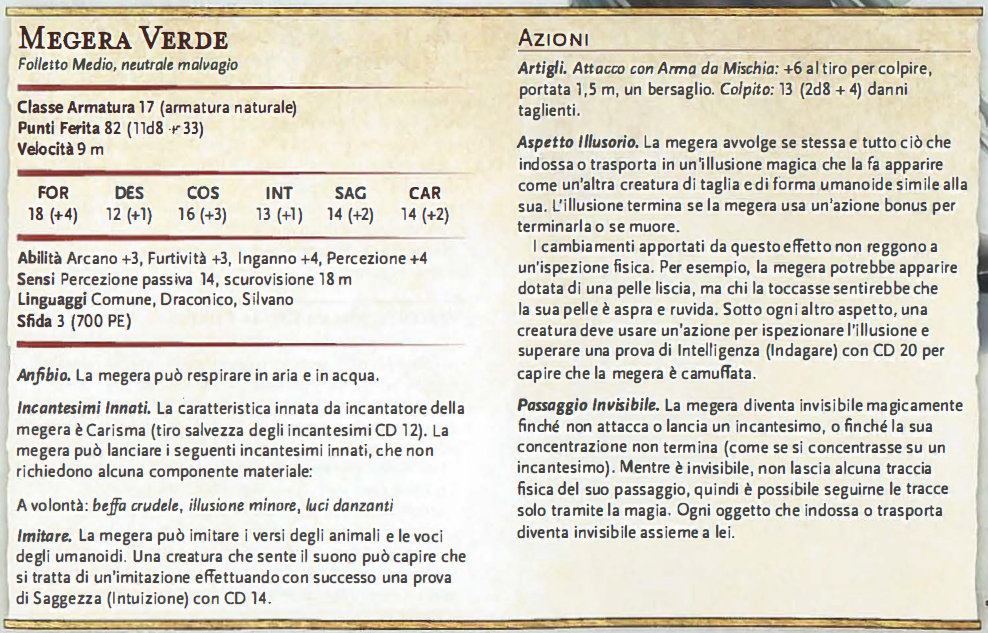
\includegraphics[width=8cm, height = 4 cm]{../Mostri/Megera_verde.png}

\section{Capitolo 8}
\begin{itemize}
    \item Il gruppo arriva finalmente a destinazione, ma scopre che Château Roquefort non esiste e non è mai esistito.
    \item Si recano alla taverna più vicina per trovare ospitalità per la notte.
    \item Larrs Thurbald, il locandiere della Trota Sballata, si interessa molto al formaggio e offre un ottimo prezzo.
    \item I Chwinga, ora soddisfatti, lasciano il formaggio ed esplorano il nuovo ambiente.
    \item Una prova con CD media permette di individuare un Chwinga mentre lascia il formaggio.
    \item A discrezione del DM, i Chwinga possono rivelarsi e ringraziare il gruppo con una Benedizione o l'anello bardico.
    \item In alternativa, possono benedire i personaggi in segreto, lasciandoli ignari della loro origine.
    \item Il locandiere serve il formaggio e tutti lo trovano delizioso.
    \item Un intenditore locale lo identifica come la cagliata vincitrice di un concorso, rubata settimane fa e dal grande valore.
    \item Tutti gli sguardi si posano sospettosi su Larrs Thurbald.
    \item Il gruppo deve decidere se difenderlo raccontando la loro improbabile storia o sgattaiolare fuori dalla città.
\end{itemize}


\section{Benedizione Chwinga}
\begin{enumerate}
    \item Benedizione del fuco amico: Hai vantaggio sui tiri di carisma quando si tenta di fare amicizia con qualcuno o di guadagnarne la fiducia.
    \item Benedizione dell’ape cercatrice: Hai vantaggio su investigazione e percezione ogni volta che cerchi tesoro.
    \item Benedizione della lingua melliflua: Hai vantaggio su carisma ogni volta che si usa una storia, una canzone o una danza interpretativa per cercare di influenzare qualcuno.
    \item Benedizione del formaggiologo: Hai una profonda conoscenza di tutto ciò che riguarda il formaggio. Sei in grado di collegare quasi tutto sotto il sole a qualche interessante curiosità sul formaggio.
    \item Benedizione dell’ape operaia: La tua operosità diventa quasi sovrumana e sei in grado di svolgere compiti al doppio della velocità che faresti normalmente, fino a un massimo di cinque volte al giorno.
    \item Benedizione dell’alveare infernale: Le vespe infernali ti considerano un amico e non ti attaccheranno. Potrebbero persino portarti dei regali. Che tu voglia il tipo di regali che portano le vespe infernali è un'altra questione...
\end{enumerate}

\end{document}
